\subsection{Test tools}
This section outlines the different test tools used - or to be used - in testing the application. 
% -------------------------------------------------------------------------
\subsubsection{Git - Source Control}
Git along with a private BitBucket account was used to source control all changes made to the original source code as well as committing individual changes and developments made to the test suite throughout developments. Changes were pushed upstream ensuring no risk of loss to progress made. Additionally, the tool is invaluable in situations where new changes break an existing reliable structure and a revert to the old state is required. 
\par 
In case the developers have not used source control as part of their workflow, we would strongly urge them to. 

\begin{figure}[H]
\centering
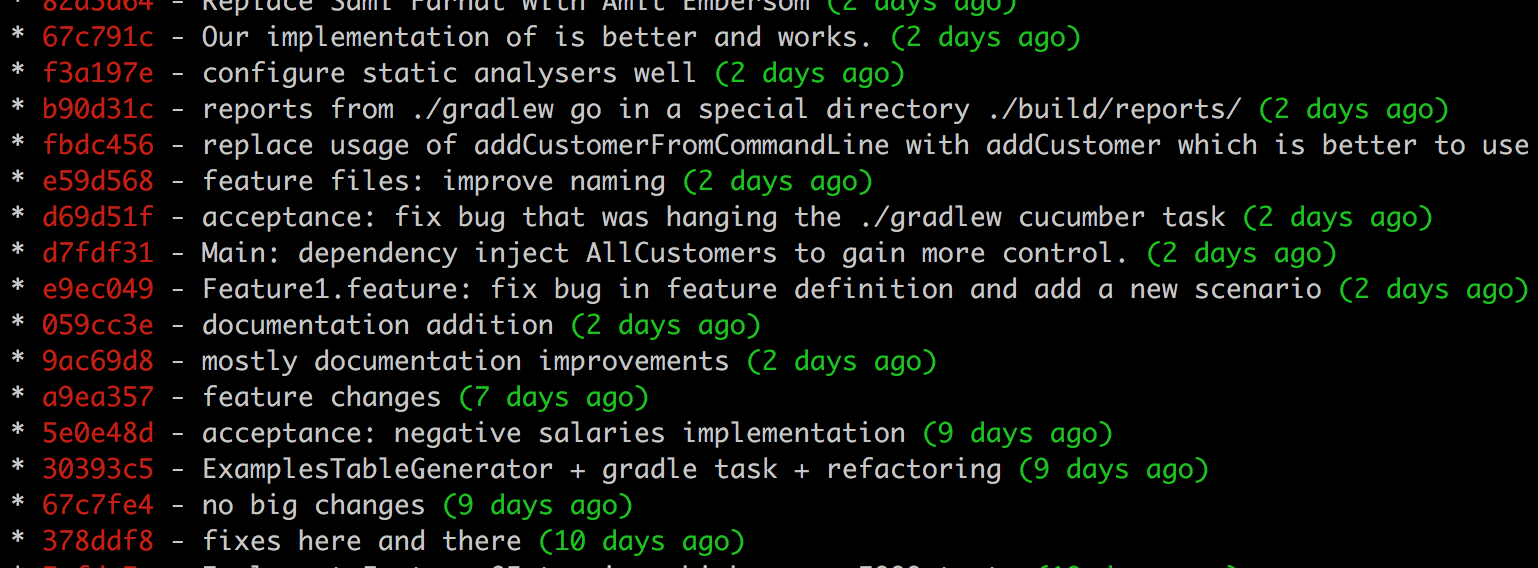
\includegraphics[scale=0.5]{res/git-tree.png}
\caption{Git-tree}
\end{figure}
% -------------------------------------------------------------------------
\subsubsection{Gradle - Build automation}
Gradle is a build automation and dependency management system often used for Java projects, providing similar functionality to Apache’s Maven and Ant. 
Gradle projects can be created by placing build.gradle file in the root of the project and defining the plugins and tasks to run. 
The tool's aptness at establishing dependency trees and the flexibility it provides in configuring new and existing tasks, allowed us to set-up convenient automations that made for a smoother testing experience. 
\par
An example of the tasks that can be run with the tool: 
\begin{itemize}
    \item \lstinline{./gradlew generate_table} is a custom task created to generate "customer tables" used in feature files. This task runs a Java executable ExamplesTableGenerator.
    \item \lstinline{./gradlew test} to run JUnit test suite 
    \item \lstinline{./gradlew cucumber} to run cucumber test suite 
    \item \lstinline{./gradlew jacocoTestReport} creates coverage reports from both JUnit and cucumber test suites. This task will run the former two to ensure most up-to-date coverage information. 
    \item \lstinline{./gradlew check} runs all static analysers (see section xx) as well as the test task. 
    \item \lstinline{./gradlew build} runs the previous check task as all compilation and setup required.  
\end{itemize}
% -------------------------------------------------------------------------
\subsubsection{Jacoco - Code Coverage}
Code coverage provides a useful metric on which classes, methods and lines of code have been executed in the application under test. 
The metric is typically monitored by test managers who would attempt to ensure it does not fall fall below a pre-set threshold value; the end aim being to maintain the amount of testing the software has undergone, increasing its  reliability (or perceived reliability).  
\par
Gradle tasks have been configured to allow for the generation of coverage reports following the run of the Cucumber and JUnit suites. The jacoco plugin works by reading files (cucumber.exec and test.exec) and generating HTML reports from them. This can be achieved by running: 
\lstinline{./gradlew jacocoTestReport} which runs the cucumber and JUnit tests before generating the reports which are placed in build/reports/jacoco/. 
\par 
The achieved code coverage from cucumber tests is 88\%. 
When both Cucumber and JUnit are run the total coverage rises to 91\%. These values are deemed satisfactory but can certainly be further increased in the future.
\begin{figure}[H]
\centering
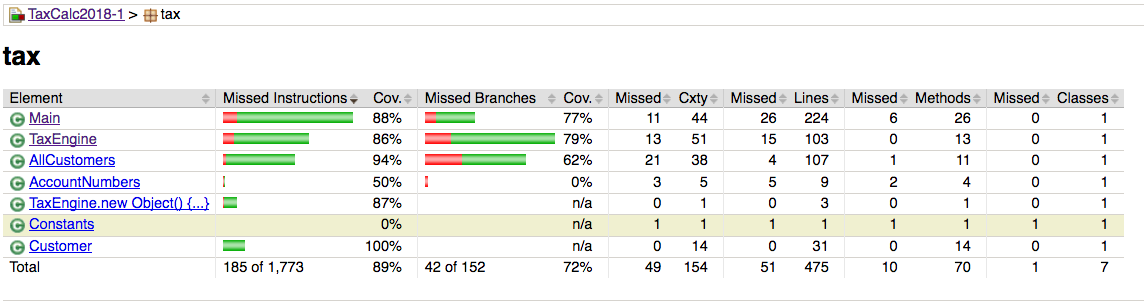
\includegraphics[scale=0.4]{res/cucumber-coverage.png}
\caption{Jacoco Code Coverage from Cucumber tests}
\end{figure}
% -----------------------------------------------------------------------
\subsubsection{Jenkins - Continuous Integration}
Continuous integration is a practice in software development to continuously combine all developers’ changes into the main repository several times per day, and run a set of predefined checks to ensure the changes made do not break existing functionality and pre-set standards. 
\par
Doing so means each developer has a near-latest sane copy of the code before making changes allowing for a reduction in the effort expended in tracking defects between different commits  
\par
In doing continuous integration, code changes pushed to the main repository  trigger the CI system to execute the steps defined in the pipeline.
Such steps may include but are not limited to: building the different executables (main and test applications), running unit test suites, acceptance test suites, static analysers (code quality and style checkers) as well as any other defined gradle, shell or other scripts.  
\par
For this project, we setup several Jenkins pipelines which are triggered upon each commit of the code. There are many ways to trigger builds in Jenkins, one such way is to continuously poll the repository for changes. 
Another is to trigger the build manually using HTTP POST. In our test implementation we have written a script found in (scripts/trigger\_jenkins.sh)to trigger the build manually using curl, a Linux tool. The script is run after every commit made. 
\begin{itemize}
    \item TaxCalc-build
	\item TaxCalc-test-acceptance
	\item TaxCalc-test-unit
\end{itemize}

\begin{figure}[H]
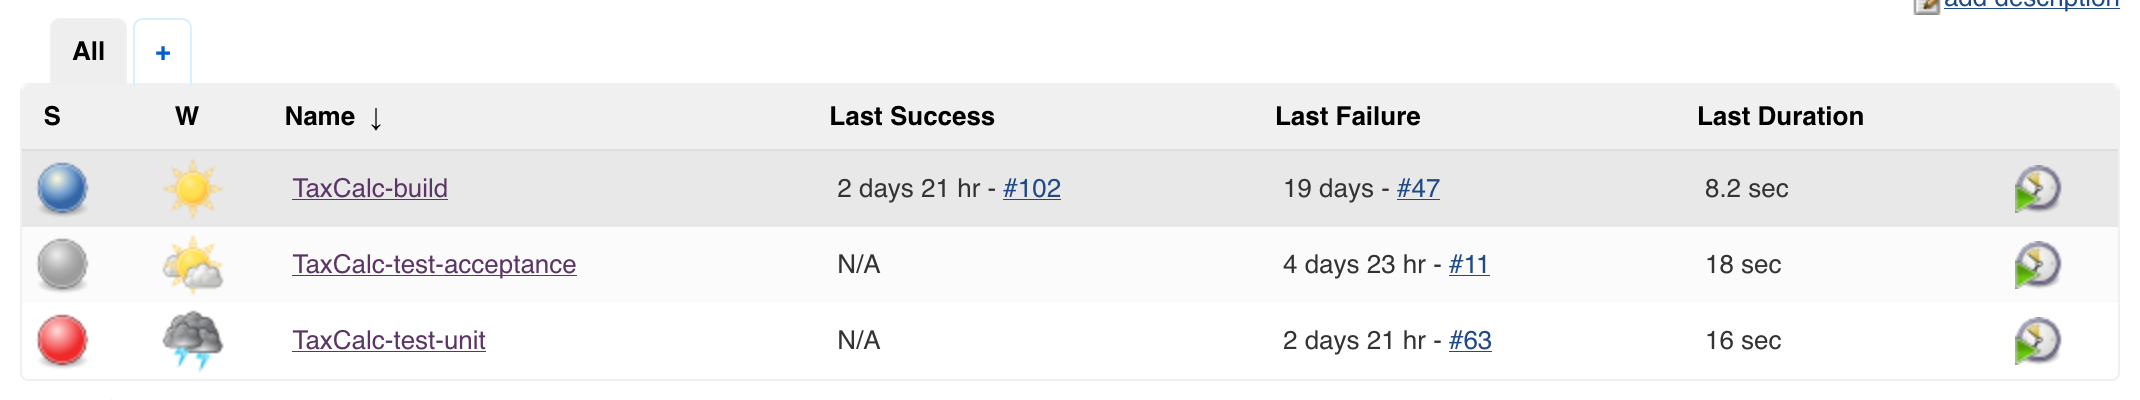
\includegraphics[scale=0.4]{res/jenkins.png}
\label{fig:jenkins-screenshot}
\caption{Screen-shot: Jenkins Project}
\end{figure}
% -----------------------------------------------------------------------
\subsubsection{Bugzilla - Defect Management}
